% Internal Physical Review Research working draft -- NOT FOR SUBMISSION.
% Submission metadata and final headline wording remain gated by resolved
% 2D/3D evidence, overlap disclosure, and explicit author approval.
\documentclass[aps,physrev,reprint,amsmath,amssymb,longbibliography,floatfix]{revtex4-2}

% Suppress pdfTeX's path/time-derived trailer ID; the clean-build wrapper
% separately verifies byte-identical output in two fresh directories.
\ifdefined\pdftrailerid
  \pdftrailerid{}
\fi

\usepackage{cmap}
\usepackage[T1]{fontenc}
\usepackage{lmodern}
\usepackage{graphicx}
\usepackage{bm}
\usepackage{booktabs}
\usepackage{hyperref}
\hypersetup{
  hidelinks,
  pdftitle={Conserved-reactivity control of encounter-time modality: weak-reaction theory and continuum-kernel designs},
  pdfauthor={Xiaoxiao Zhouyi and Luca Giuggioli},
  pdfsubject={Internal research draft on multimodal encounter-reaction times},
  pdfkeywords={encounter reaction, reaction-time density, multimodality, conserved reactivity, fold, cusp}
}
\usepackage{placeins}

\graphicspath{{../artifacts/figures/}}
\renewcommand{\topfraction}{0.92}
\renewcommand{\textfraction}{0.05}
\renewcommand{\floatpagefraction}{0.82}

\newcommand{\dd}{\mathrm d}
\newcommand{\e}{\mathrm e}
\newcommand{\Lfree}{\mathcal L}
\newcommand{\Tkill}{\mathcal T_{\kappa}}
\newcommand{\budget}{\mathcal B}
\newcommand{\status}[1]{\textbf{[#1]}}
% Generated by code/build_manuscript_inputs.py; do not edit by hand.
% numerical-source manifest SHA-256: 6ea29628e1cba423d37588b72a78dd3f5934f5e77b9c83df70394739375c88e7
% four-patch SHA-256: 4a929cdaf915a9b6180acc0c272a16ae77087d097f2d078b6483c6c9b320a9fc
% physical-d=3 four-patch SHA-256: 125234df2817287c30699d80e30af0e711c036193f0a64a404c8f3e98f98f984
% G1c SHA-256: cce1e34c599564dc932da6af4d4146c2c396836990e9b51414fc2f843e123bb4
% G1d SHA-256: 268e3f988330a2f28ad79b22cdf1f7e53a0142dc007d2a2a7cbfe40d18f91f92
% broad-patch B=0 bridge SHA-256: 6a18e668401ae5776eebd7bd58c7bd553838db21998efdba2865cea094ae207b
\providecommand{\FourPatchCuspTime}{13.3280319895}
\providecommand{\FourPatchCuspWeights}{0.28000000,0.23019485,0.20932396,0.28048119}
\providecommand{\FourPatchMaxResidual}{1.10\times10^{-12}}
\providecommand{\FourPatchScaledFourth}{-42.8118}
\providecommand{\FourPatchSvdRatio}{0.256405}
\providecommand{\FourPatchSelectedStep}{0.11}
\providecommand{\FourPatchSelectedWeights}{0.28000000,0.26950477,0.10658775,0.34390748}
\providecommand{\FourPatchRootOne}{3.20404}
\providecommand{\FourPatchRootTwo}{5.08547}
\providecommand{\FourPatchRootThree}{8.68847}
\providecommand{\FourPatchRootFour}{13.32803}
\providecommand{\FourPatchRootFive}{22.66010}
\providecommand{\FourPatchPeakRatio}{0.85413}
\providecommand{\FourPatchValleyOne}{0.66679}
\providecommand{\FourPatchValleyTwo}{0.83754}
\providecommand{\FourPatchCuspTimeSpread}{1.43\times10^{-11}}
\providecommand{\FourPatchWeightSpread}{1.05\times10^{-14}}
\providecommand{\FourPatchFourthDifference}{8.84\times10^{-9}}
\providecommand{\FourPatchPolarDifference}{6.60\times10^{-15}}
\providecommand{\FourPatchRootDifference}{7.11\times10^{-15}}
\providecommand{\DThreeCuspTime}{12.8097399605}
\providecommand{\DThreeCuspWeights}{0.28000000,0.18220393,0.20766999,0.33012608}
\providecommand{\DThreeCuspWeightOne}{0.28000000}
\providecommand{\DThreeCuspWeightTwo}{0.18220393}
\providecommand{\DThreeCuspWeightThree}{0.20766999}
\providecommand{\DThreeCuspWeightFour}{0.33012608}
\providecommand{\DThreeScaledFourth}{-39.8723}
\providecommand{\DThreeSvdRatio}{0.240300}
\providecommand{\DThreeSelectedStep}{0.10}
\providecommand{\DThreeSelectedWeights}{0.28000000,0.21134977,0.11201164,0.39663859}
\providecommand{\DThreeSelectedWeightOne}{0.28000000}
\providecommand{\DThreeSelectedWeightTwo}{0.21134977}
\providecommand{\DThreeSelectedWeightThree}{0.11201164}
\providecommand{\DThreeSelectedWeightFour}{0.39663859}
\providecommand{\DThreeRootOne}{3.07471}
\providecommand{\DThreeRootTwo}{5.50128}
\providecommand{\DThreeRootThree}{8.26705}
\providecommand{\DThreeRootFour}{12.80974}
\providecommand{\DThreeRootFive}{21.46418}
\providecommand{\DThreePeakRatio}{0.63381}
\providecommand{\DThreeValleyOne}{0.76924}
\providecommand{\DThreeValleyTwo}{0.84480}
\providecommand{\DThreeSphericalDifference}{1.08\times10^{-14}}
\providecommand{\DThreeCuspTimeDifference}{1.28\times10^{-11}}
\providecommand{\DThreeWeightDifference}{1.50\times10^{-14}}
\providecommand{\DThreeFourthDifference}{4.05\times10^{-10}}
\providecommand{\DThreeRootDifference}{6.18\times10^{-13}}
\providecommand{\DThreeEligibleCount}{11}
\providecommand{\GOneCControlCount}{66}
\providecommand{\GOneCEdgeCount}{165}
\providecommand{\GOneCSeedCount}{3}
\providecommand{\GOneCManualReviewCount}{53}
\providecommand{\GOneDFoldTime}{10.5022583145}
\providecommand{\GOneDFoldControl}{0.6388077421}
\providecommand{\GOneDFoldWeights}{0.20000000,0.06388077,0.73611923}
\providecommand{\GOneDFoldWeightOne}{0.20000000}
\providecommand{\GOneDFoldWeightTwo}{0.06388077}
\providecommand{\GOneDFoldWeightThree}{0.73611923}
\providecommand{\GOneDFoldDensity}{0.0256240551}
\providecommand{\GOneDScaledFt}{2.84\times10^{-15}}
\providecommand{\GOneDScaledFtt}{2.39\times10^{-13}}
\providecommand{\GOneDScaledFttt}{-7.9231}
\providecommand{\GOneDScaledFtlambda}{-0.32729}
\providecommand{\GOneDScaledFttlambda}{-0.61492}
\providecommand{\GOneDJacobianDeterminant}{-2.59316}
\providecommand{\BroadBZeroSelectedStep}{0.13}
\providecommand{\BroadBZeroCuspTime}{13.30724696}
\providecommand{\BroadBZeroScaledFourth}{-44.6816}
\providecommand{\BroadBZeroSvdRatio}{0.2649}
\providecommand{\BroadBZeroSelectedWeights}{0.28000,0.27737,0.08572,0.35692}
\providecommand{\BroadBZeroCuspErrors}{0.5092,0.2706,0.1519,0.0666}
\providecommand{\BroadBZeroRootErrors}{0.5337,0.2643,0.1562,0.0669}
\providecommand{\BroadBZeroFinestCuspError}{0.06662}
\providecommand{\BroadBZeroFinestRootError}{0.06685}
\providecommand{\BroadBZeroWorstValleyMargin}{0.03207}

% Generated by code/build_positive_b_manuscript_input.py; do not edit.
% manifest SHA-256: 955e59bf333b5fd70e415a53dc26becae9c7a34c5d40f1230c96b1dab8f5677c
% canonical result SHA-256: 51e8eb4bdb652124865d0c39e6f36b99d13ed61578b161e0f75b142cada49401
% two-process evidence SHA-256: 6c0eccaae09ef95923843ddd7a141a27311e1575ee68d3301b4757b785ee9890
% independent audit SHA-256: 60c541a6f0decd5431cefa5c203311176e61006586ce69043d5fcf5380ed517d
% Scope: fixed box, same FV solver family, two odd meshes, finite window.
% Forbidden: allocation cusp, continuum/unbounded, independent solver, PRR pass.
\providecommand{\PositiveBBudget}{0.01}
\providecommand{\PositiveBWeights}{0.28000000,0.27736690,0.08571723,0.35691587}
\providecommand{\PositiveBMeshOne}{113}
\providecommand{\PositiveBMeshTwo}{129}
\providecommand{\PositiveBRootTimesOne}{3.33676,5.09431,8.62228,13.56147,22.54890}
\providecommand{\PositiveBRootTimesTwo}{3.30670,5.08515,8.58848,13.52917,22.51482}
\providecommand{\PositiveBPeakRatioOne}{0.83339}
\providecommand{\PositiveBPeakRatioTwo}{0.83914}
\providecommand{\PositiveBPeakRatioRange}{0.83339\text{--}0.83914}
\providecommand{\PositiveBValleyRatiosOne}{0.78239,0.84673}
\providecommand{\PositiveBValleyRatiosTwo}{0.76468,0.84375}
\providecommand{\PositiveBBasinMassesOne}{0.00521143,0.01662829,0.14837901}
\providecommand{\PositiveBBasinMassesTwo}{0.00522784,0.01659738,0.14848157}
\providecommand{\PositiveBBasinOneRange}{0.00521143\text{--}0.00522784}
\providecommand{\PositiveBBasinTwoRange}{0.01659738\text{--}0.01662829}
\providecommand{\PositiveBBasinThreeRange}{0.14837901\text{--}0.14848157}
\providecommand{\PositiveBValleyOneRange}{0.76468\text{--}0.78239}
\providecommand{\PositiveBValleyTwoRange}{0.84375\text{--}0.84673}
\providecommand{\PositiveBFinalSurvivalOne}{0.82978127}
\providecommand{\PositiveBFinalSurvivalTwo}{0.82969321}
\providecommand{\PositiveBFinalSurvivalRange}{0.82969321\text{--}0.82978127}
\providecommand{\PositiveBMinimumBasinMass}{0.00521143}
\providecommand{\PositiveBWorstValleyRatio}{0.84673}
\providecommand{\PositiveBMaximumRootDifference}{0.03408}
\providecommand{\PositiveBMaximumMassDifference}{1.03\times10^{-4}}
\providecommand{\PositiveBFinalSurvivalDifference}{8.81\times10^{-5}}
\providecommand{\PositiveBFinalTime}{100}


\begin{document}

\title{Conserved-reactivity control of encounter-time modality:\\
weak-reaction theory and continuum-kernel designs}

\author{Xiaoxiao Zhouyi}
\email{xiaoxiao.zhouyi@bristol.ac.uk}
\author{Luca Giuggioli}
\affiliation{School of Engineering Mathematics and Technology, University of Bristol,
Bristol BS8 1TW, United Kingdom}

\date{July 13, 2026}

\begin{abstract}
\textbf{Internal status---not a submission claim.}
We study reaction-time modality under one conserved centre-space reactivity
integral.  Within each fixed comparison, only nonnegative catalyst weights
vary; transport, contact geometry, initial law, and patch supports remain
fixed.  For every fixed finite integer $d\ge2$, each fixed finite $m$, and
target times satisfying a monotone-path and contact-interior condition, we
construct a $d$- and $m$-dependent longitudinal-slab family in the exact
encounter quotient.  Here $\epsilon$
jointly scales the OU noise, initial variances, and slab width.  After first
fixing a sufficiently small $\epsilon$ and then taking a sufficiently small
positive installed budget $B$, the Doi density has at least $m$
nondegenerate maxima; extra extrema and an absolute event-mass floor are not
controlled.  A weighted-space compact-positive-time mixed-jet estimate and
explicit contraction/rank conditions give the corresponding weak-reaction
transfer.  Separately, a result-informed physical-$d=2$ $B=0$ free-exposure
calculation with four compact slabs has a nondegenerate cusp at
$t_c=\FourPatchCuspTime$ and passes declared relative-prominence shape gates
with three retained maxima.  The exact physical-$d=3$ sphere kernel, evaluated
in a separate result-informed chain, retains the same five-root topology and
passes the same relative-shape gates.  A post-G1c, result-informed calculation on one
bounded reflected $207\,025$-state finite-volume box at $B=0.6$ confirms a
nondegenerate fold at $t_f=\GOneDFoldTime$; its numerical choices were frozen
before execution, but it was not a preregistered discovery.  Neither result
is an interval-global or continuum positive-$B$ three-mode confirmation.  In
the broad physical-$d=2$ family, the allocation selected from the
$B\downarrow0$ calculation was then tested without refitting at
$B=\PositiveBBudget$.  Odd meshes $N=\PositiveBMeshOne,\PositiveBMeshTwo$ in
one fixed reflected box retain five alternating stationary roots on the saved
root screen $t\leq35$; valley-partitioned basin masses and tail checks extend
through $t=100$, and the smallest basin mass is \PositiveBMinimumBasinMass.
This does not exclude additional extrema after $t=35$.  It is a fixed-control,
same-solver point, not an interval-global result, allocation cusp, or continuum
limit.  Submission remains gated by the same-family finite-$B$
cusp and folds, parity/alignment/box continuation, and an independent
killed-process calculation; positive-$B$ physical-$d=3$ evidence is also
required for a two-/three-dimensional headline.
\end{abstract}

\maketitle

\section{Question, evidence levels, and non-overlap}\label{sec:intro}

First-passage and reaction-time densities can be multimodal when distinct
trajectory families reach a reactive set on separated time scales
\cite{godecMetzler2017twochannel,grebenkovMetzlerOshanin2018defocusing}.
Strategically placed absorbing traps already produce multimodal continuum
capture densities in two dimensions \cite{lindsaySpoonmoreTzou2016narrow},
and two-mobile-particle encounter densities have been resolved in physical
dimensions two and three, including two-hump cases
\cite{leVotEtAl2022encounter}.  Exact lattice and network studies, including
work by Giuggioli and co-workers, provide further multipeak mechanisms driven
by transport structure or disorder
\cite{giuggioliPerezBeckerSanders2013,giuggioli2020confined,
giuggioliEtAl2024multitarget,marrisEtAl2025disordered}.

Within each fixed control family, the unreactive transport, geometry, contact
scale, initial law, and patch supports are held fixed.  The sole control is a
static spatial Doi reactivity field whose installed amount is conserved.
Spectral survival theory for spatially
distributed volumetric traps already resolves how trap arrangement changes
reaction rates \cite{nguyenGrebenkov2010porous}.  General heterogeneous-Robin reaction-time
theory already exists \cite{grebenkov2019heterogeneous}, as does fixed-total-
reactivity optimization for steady flux \cite{nicolaouMulder2023flux} and
encounter-history or local-time reaction theory
\cite{grebenkov2007residence,grebenkov2020multiple,
grebenkov2020paradigm}.  We therefore claim none of those individual
ingredients as new.  We target their intersection with timing-modality
control and model-specific bifurcation geometry.  A targeted primary-source
search did not locate this complete chain; that search is not proof of
absence.

We use one evidence ontology:
\status{proved}, \status{numerically verified---reduced},
\status{numerically verified---discrete diagnostic},
\status{numerically confirmed---exact free-exposure kernel}, \status{conjectural},
\status{implementation smoke pass}, \status{mathematical no-go}, and
\status{project gate failed}.
A software or reproducibility pass is never relabeled as a scientific pass.

This internal project follows two related working manuscripts in the same
research program.  One develops finite encounter-reaction reductions and
reduced-clock screening; the other develops finite-state localized-delivery
response and catastrophe examples.  Public identifiers, editor-facing copies,
and an author-approved equation/code/data/figure overlap map remain release
gates.  Neither related manuscript is used as independent validation here.
Consequently no novelty is claimed for Duhamel's identity, catastrophe normal
forms, generic fold powers, a first fold, or a first cusp.  The non-overlapping
target chain is
\begin{equation}
\begin{split}
&\text{fixed-budget multi-rate jet control}\\
&\quad\longrightarrow\text{sufficient at-least-}m\text{ channel design}\\
&\quad\longrightarrow\text{model-specific continuum jet realization}.
\end{split}
\label{eq:chain}
\end{equation}

The strongest existence statement below concerns any prescribed fixed finite
$m$ in a $d$- and $m$-dependent physical slab family for every fixed finite
integer $d\ge2$.  It is pointwise rather than uniform in $d$ and $m$, and is
not a $d\to\infty$ or uniform $m\to\infty$ limit, or an assertion
that one fixed spatial configuration has arbitrarily many modes.  The exact
$B=0$ kernel shapes below are finite-parameter confirmations in both
dimensions.  One unchanged broad physical-$d=2$ allocation also has
event-mass-qualified modes at positive budget on two odd meshes in a fixed
box.  Allocation-cusp control, parity/alignment/box continuation, and an
independent killed-process method remain separate publication gates.

\section{Continuum model and one physical budget}\label{sec:model}

Let $q(z,t)$ be the unreacted two-particle configuration density in the Doi
volume-reaction model \cite{doi1976stochastic}, where
$z=(x_1,x_2)$.  The fixed conservative transport generator is $\Lfree$.
Write $r=x_1-x_2$ and let $c=C_\eta(x_1,x_2)$ be the declared physical
encounter-centre coordinate.  With a fixed contact profile $\chi_a$ and fixed
smooth centre patches $\phi_j$, define
\begin{align}
 \kappa_{\bm w}(c)&=B\sum_{j=1}^{J}w_j\phi_j(c),
 &w_j&\ge0,\nonumber\\
 \sum_jw_j&=1,
 &\int_{\mathcal C}\phi_j(c)\,\dd c&=1,\nonumber\\
 K_{\bm w}(z)&=\chi_a(r)\kappa_{\bm w}(c).
\label{eq:field}
\end{align}
The conserved installed-catalyst functional is
\begin{equation}
 \mathcal C(\kappa_{\bm w})
 =\int_{\mathcal C}\kappa_{\bm w}(c)\,\dd c=B.
\label{eq:budget}
\end{equation}
It is not the integral of $K_{\bm w}$ over two-particle configuration space,
a stationary-exposure weighting, or a number of reactive grid states.  For an
unnormalized basis the cost covector is
$c_j=\int_{\mathcal C}\phi_j(c)\,\dd c$, and budget-tangent perturbations obey
$\bm c^{\mathsf T}\bm h=0$.

The killed generator, state, reaction-time density, and mass balance are
\begin{align}
 \Tkill&=\Lfree-M_{K_{\bm w}},
 & q(t)&=\e^{t\Tkill}q_0,\nonumber\\
 f(t;\bm w)&=\langle K_{\bm w},q(t)\rangle,
 &-\frac{\dd}{\dd t}\langle1,q(t)\rangle&=f(t;\bm w).
\label{eq:massbalance}
\end{align}
All supports, transport coefficients, contact radius, and the initial law are
fixed while $\bm w$ varies.  This is an amplitude-control problem, not a shape
derivative for moving masks.

\section{A reduced design lemma and its ancestry}\label{sec:gig}

A related encounter manuscript uses generalized-inverse-Gaussian (GIG) clocks
\cite{barndorffNielsenEtAl1978gig} for reduced screening.  For $p>1$, $b>0$,
and $A_j>0$, write
\begin{equation}
 g_j(t)=Z_j^{-1}t^{-p}
 \exp\!\left(-\frac{A_j}{t}-bt\right),\qquad t>0.
\label{eq:gig}
\end{equation}
Taking $m_j=m_0R^{j-1}$, $A_j=bm_j^2+pm_j$, and mixture weights inversely
proportional to $g_j(m_j)$ makes every isolated peak occur at $m_j$.  For
each fixed finite $m,p$, and $bm_0$, separation estimates give a finite
$R_{\rm sep}$ such that $R\ge R_{\rm sep}$ yields at least $m$
nondegenerate maxima.  This supporting reduced lemma is \status{proved}; it
does not give the smallest threshold, exclude extra critical points, or
establish event mass.  The $p=2.5$, $b=0.01$, $R=10$, $m=2,\ldots,6$ root
screen and the three-clock cusp are \status{numerically verified---reduced}
diagnostics inherited from that screening program, not new physical evidence
in this paper.  GIG probabilities are not identified with the physical
catalyst weights in Eq.~\eqref{eq:field}.

\section{Fixed-budget response and exact modality jets}\label{sec:response}

For a fixed-support perturbation $H$, Duhamel's identity gives
\begin{align}
D_\kappa f(t)[H]
={}&\langle H,\e^{t\Tkill}q_0\rangle\nonumber\\
&-\int_0^t
\left\langle K_{\bm w},
\e^{(t-s)\Tkill}M_H\e^{s\Tkill}q_0\right\rangle\dd s.
\label{eq:duhamel}
\end{align}
This exact identity is shared background.  The multi-rate object needed here
is a projected jet map.  For target observables
$Y_a=\partial_t^{r_a}f(t_a;\bm w)$, define
$G_{aj}=\partial_{w_j}Y_a$ and choose a local control metric $M\succ0$.
For a general cost covector $\bm c$,
\begin{equation}
 \widetilde G
 =G-\frac{(GM^{-1}\bm c)\bm c^{\mathsf T}}
 {\bm c^{\mathsf T}M^{-1}\bm c}.
\label{eq:projectedG}
\end{equation}
If the control lies in the simplex interior and
$\operatorname{rank}\widetilde G=q$, the unique budget-preserving perturbation
of minimum $M$-norm that realizes a target infinitesimal jet $\bm y$ is
\begin{equation}
 \bm h_*
 =M^{-1}\widetilde G^{\mathsf T}
 (\widetilde GM^{-1}\widetilde G^{\mathsf T})^{-1}\bm y.
\label{eq:multijet}
\end{equation}
Equations~\eqref{eq:projectedG}--\eqref{eq:multijet} are
\status{proved} constrained linear algebra.  They are local, not a global
finite-amplitude control theorem.  A physical controllability claim still
requires a continuum-stable positive lower bound on
$\sigma_{\min}(\widetilde GM^{-1/2})$.

Writing $F=f_t$, a nondegenerate one-control fold satisfies
\begin{equation}
 f_t=f_{tt}=0,\qquad
 f_{ttt}f_{t\theta}\ne0.
\label{eq:fold}
\end{equation}
Its minimal persistence jet is
\begin{equation}
 \mathcal J_{\rm fold}
 =\{f_t,f_{tt},f_{ttt},f_{t\theta},f_{tt\theta}\}.
\label{eq:foldjet}
\end{equation}
With two independent budget controls, a cusp satisfies
\begin{equation}
 f_t=f_{tt}=f_{ttt}=0,\qquad f_{tttt}\ne0,
\label{eq:cusp}
\end{equation}
and the projected gradients of $f_t$ and $f_{tt}$ have rank two.  Its exact
persistence jet is
\begin{equation}
\begin{split}
\mathcal J_{\rm cusp}=\{&
 f_t,f_{tt},f_{ttt},f_{tttt},\\
 &f_{t\theta_i},f_{tt\theta_i},f_{ttt\theta_i}:i=1,2\}.
\end{split}
\label{eq:cuspjet}
\end{equation}
Full joint $C^3$ and $C^4$ convergence are convenient sufficient conditions
for the fold and cusp, respectively.  A cusp creates only one additional
local max--min pair.  A trimodal conclusion also needs a remote pair with
uniform root, curvature, prominence, and tail margins.

\section{Weak-reactivity continuum bridge and remaining global target}
\label{sec:bridge}

Write $K_{B,\bm w}=BV_{\bm w}$ and
$A_{B,\bm w}=\Lfree-BM_{V_{\bm w}}$.  First let $\mathcal Q_{\rm box}$ be a
bounded Lipschitz quotient with reflecting boundaries and a reversible free
invariant density bounded above and below.  The free forward operator is then
similar to a nonpositive self-adjoint weighted-Neumann operator.  Bounded
indicator killing preserves an analytic semigroup.  For $q_0\in L^2$ every
finite time/control mixed jet exists on
$[\tau,T]$, $\tau>0$, even though the contact indicator is discontinuous.
If $w(\bm\theta)=w_*+P\bm\theta$ and $U_i=V_{P\bm e_i}$, the first two exact
state sensitivities satisfy
\begin{align}
 \partial_t s_i&=A_{B,\bm w}s_i-BU_iq,&s_i(0)&=0,\nonumber\\
 \partial_t s_{ij}&=A_{B,\bm w}s_{ij}-BU_is_j-BU_js_i,
 &s_{ij}(0)&=0.
\label{eq:sensitivitypde}
\end{align}
The observable must also be differentiated.  In particular,
\begin{align}
 \partial_i f_B&=B\{\langle U_i,q\rangle
                  +\langle V_{\bm w},s_i\rangle\},\nonumber\\
 \partial_{ij}f_B&=B\{\langle U_i,s_j\rangle+\langle U_j,s_i\rangle
                  +\langle V_{\bm w},s_{ij}\rangle\}.
\label{eq:directterms}
\end{align}
Omitting the direct terms in Eq.~\eqref{eq:directterms} gives the wrong
control jet.  Perturbative treatments of spatially nonuniform partial
absorption precede this calculation \cite{ryu2009inhomogeneous,
ryuJohnson2009nonuniform}; the object used here is the transient,
budget-projected mixed time/control jet.

The analytically tractable leading object is the normalized density and its
free-exposure limit,
\begin{equation}
 F_B(t,\bm\theta)=B^{-1}f_B(t,\bm\theta),\qquad
 G(t,\bm\theta)=\langle V_{\bm w(\bm\theta)},
 \e^{t\Lfree}q_0\rangle.
\label{eq:freeexposure}
\end{equation}
The reactivity-times-occupancy identity and its occupation-time/local-time
interpretations are standard
\cite{pruestelMeierSchellersheim2014area,bressloff2022feynmanKac,
grebenkov2007residence,grebenkov2020multiple}; here they provide the
budget-normalized leading object rather than a new reaction formalism.
Let $\Theta$ be a compact interior control set and let $\Theta_\delta$ be a
complex control tube.  With
$v_{\infty,\delta}=\sup_{\Theta_\delta}\|V_{\bm w}\|_\infty$,
$v_{2,\delta}=\sup_{\Theta_\delta}\|V_{\bm w}\|_2$, and $\kappa_\pi$ the
reversible-similarity condition number, Dyson expansion followed by
time/control Cauchy estimates gives, for every fixed $r$ and multi-index
$\alpha$,
\begin{align}
&\sup_{[\tau,T]\times\Theta}
\left|\partial_t^r\partial_{\bm\theta}^{\alpha}(F_B-G)\right|
\nonumber\\
&\quad\le r!\alpha!\left(\frac{2}{\tau}\right)^r
\delta^{-|\alpha|}v_{2,\delta}\kappa_\pi\nonumber\\
&\qquad\times
\left[\e^{(3/2)Bv_{\infty,\delta}T}-1\right]\|q_0\|_2
=O(B).
\label{eq:weakbridge}
\end{align}
This is a \status{proved} compact-positive-time continuum mixed-jet bridge.
The first Dyson correction has an explicit $O(B^2)$ remainder on the same
complex neighborhood.

\paragraph{Unbounded weighted-space corollary.}
For the physical cylinder
$\mathcal Q_d^\infty=\mathbb R^2\times\mathbb T_W^{d-1}$, let $\pi$ be the
Gaussian--uniform reversible invariant density and set
\begin{equation}
 X_\pi=L^2(\pi^{-1}\dd x),\qquad
 \|V\|_{X_\pi^*}=\|V\|_{L^2(\pi\dd x)}.
\label{eq:weightedspace}
\end{equation}
The map $u\mapsto q=\pi u$ is unitary from $L^2(\pi\dd x)$ to $X_\pi$.
Thus, for $q_0\in X_\pi$ and bounded fixed-$\epsilon$ killing profiles, the
same proof gives Eq.~\eqref{eq:weakbridge} with $\kappa_\pi=1$,
$v_{2,\delta}$ replaced by
$\sup_{\Theta_\delta}\|V_{\bm w}\|_{X_\pi^*}$, and $\|q_0\|_2$ replaced by
$\|q_0\|_{X_\pi}$.  This is the version used by the unbounded-cylinder
theorem below; it is not obtained from a bounded-box similarity constant.

\paragraph{Quantitative persistence criterion.}
With the continuous extension $F_0=G$, let
$H_B=(F_{B,t},F_{B,tt})$ for a fold, with variables
$x=(t,\theta)$, or let
$H_B=(F_{B,t},F_{B,tt},F_{B,ttt})$ for a cusp, with variables
$x=(t,\theta_1,\theta_2)$.  Suppose $H_0(x_0)=0$,
$A_0=DH_0(x_0)$ is invertible, and the closed ball
$\overline{B_r(x_0)}$ lies inside positive time and the simplex interior.  If
\begin{align}
 \sup_{x\in\overline{B_r(x_0)}}
 \|I-A_0^{-1}DH_B(x)\|_2&\le\tfrac12,\nonumber\\
 \|A_0^{-1}H_B(x_0)\|_2&\le\tfrac r2,
\label{eq:contractioncriterion}
\end{align}
then $x\mapsto x-A_0^{-1}H_B(x)$ is a contraction of the ball into itself.
It has one zero $x_B$ there,
\begin{equation}
 \|x_B-x_0\|_2\le
 2\|A_0^{-1}H_B(x_0)\|_2,
\label{eq:displacement}
\end{equation}
 and $DH_B(x_B)$ remains invertible.  For a cusp, or any unfolding with at
least two simplex-tangent controls, nondimensionalize time once and use one
frozen dimensionless tangent metric.  In that metric define the two-row
projected control response
\begin{equation}
 R_B(x)=
 \begin{pmatrix}
  \nabla_{\bm\theta}(F_B)_t(x)\\
  \nabla_{\bm\theta}(F_B)_{tt}(x)
 \end{pmatrix},
\label{eq:weylrank}
\end{equation}
with $R_0$ defined by $F_0=G$.  On
$U=\overline{B_r(x_0)}$, suppose
\begin{align}
 s_*&:=\inf_{x\in U}\sigma_2(R_0(x))>0,\nonumber\\
 \varepsilon_R(B)&:=\sup_{x\in U}\|R_B(x)-R_0(x)\|_2<s_*.
\label{eq:weylregion}
\end{align}
Weyl's inequality then gives
$\inf_{x\in U}\sigma_2(R_B(x))\ge s_*-\varepsilon_R(B)>0$, including at the
displaced root $x_B$.  The finite collection of entrywise bounds from
Eq.~\eqref{eq:weakbridge} controls $\varepsilon_R(B)$.  The raw response for
$f_B$ is $B R_B$: normalized rank can persist while its absolute smallest
singular value and the event rate vanish as $B\downarrow0$.
For a one-control fold, Eq.~\eqref{eq:contractioncriterion} and the resulting
invertibility of $DH_B(x_B)$ supply the local transfer; no rank-two condition
is imposed on its $2\times1$ control response.  For a cusp, the contraction
criterion together with Eqs.~\eqref{eq:weylrank}--\eqref{eq:weylregion} and
the nonzero quartic margin supplies the explicit small-$B$ transfer conditions.

For the exact slab quotient, the free clocks factor as
$g_j(t)=a_j(t)c_d(t)$.  With $g=(g_1,g_2,g_3)^{\mathsf T}$, define
\begin{equation}
 \mathcal D(t)=
 \begin{pmatrix}g'(t)^{\mathsf T}\\g''(t)^{\mathsf T}\\
 g'''(t)^{\mathsf T}\end{pmatrix},\qquad
 \Delta(t)=\det\mathcal D(t).
\label{eq:freedeterminant}
\end{equation}
Analytical modality criteria for finite mixtures are classical
\cite{rayLindsay2005topography}; the following Wronskian-like determinant and
its conserved-simplex identity are specific to the present encounter clocks.
A rank-two zero of $\Delta$ whose normalized null vector $\bm w_*$ is strictly
positive is an interior free-exposure cusp provided
$g''''(t_*)^{\mathsf T}\bm w_*\ne0$ and the two budget-tangent rows
$g'(t_*)^{\mathsf T}P,g''(t_*)^{\mathsf T}P$ have rank two.  The exact
identity
\begin{align}
 \det DC_0(t_*,0)
 &=[g''''(t_*)^{\mathsf T}\bm w_*]\nonumber\\
 &\quad\times
 \det\!\begin{pmatrix}g'(t_*)^{\mathsf T}P\\g''(t_*)^{\mathsf T}P\end{pmatrix}
 \nonumber\\
 &=\det[P,\bm w_*]\,\Delta'(t_*)
\label{eq:cuspdetidentity}
\end{align}
turns spatial configuration into a computable cusp-design criterion.  These
standard ingredients provide a model-specific route from a quantified
free-exposure singularity to a nearby weak-Doi singularity.  A finite-budget,
event-mass-qualified fixed-control point is given below; establishing the
same-family cusp, both folds, and their converged continuation remains a
separate gate.

The theorem is not uniform on the long scale $t=O(B^{-1})$, does not show that
the pilot value $B=0.6$ is small, and does not by itself exclude late extra
critical points.  Event mass on a fixed window is $O(B)$, so an observability
lower bound must overlap the theorem's small-$B$ upper bound.  A
Scharfetter--Gummel/FEM $C^1$ jet estimator and an independent solver remain
separate gates.

\subsection{Direct fixed-finite-mode theorem in every fixed finite $d\ge2$}

The GIG family is not needed to prove physical existence.  Fix
$d\in\mathbb N$ with $d\ge2$, $D_0,\gamma,W,\rho,s_0,u_0>0$,
$0<a<W/2$, and
$z_0\ne\bar z$, and let the longitudinal midpoint satisfy
\begin{equation}
\begin{aligned}
 \dd Z_t&=-\gamma(Z_t-\bar z)\,\dd t
          +\epsilon\sqrt{D_0}\,\dd W_t,\\
 Z_0&\sim N(z_0,\epsilon^2s_0^2),\\
 \mu(t)&=\bar z+(z_0-\bar z)\e^{-\gamma t}.
\end{aligned}
\label{eq:narrowou}
\end{equation}
For the relative quotient of two independent equal-diffusivity walkers, use
\begin{align}
 \dd R_{\parallel,t}&=-\gamma R_{\parallel,t}\,\dd t
 +2\epsilon\sqrt{D_0}\,\dd W_{\parallel,t},\nonumber\\
 \dd R_{\perp,t}&=2\epsilon\sqrt{D_0}\,\dd\bm W_{\perp,t}
 \pmod W,\nonumber\\
 R_{\parallel,0}&\sim
 N(r_{\parallel,0},\epsilon^2u_0^2),\nonumber\\
 R_{\perp,0}&\sim \operatorname{WN}
 (r_{\perp,0},\epsilon^2\Sigma_{\perp,0}),
\label{eq:relativequotient}
\end{align}
where $\operatorname{WN}$ denotes a wrapped Gaussian on the transverse torus
and $r_{\perp,0}\in\mathbb T_W^{d-1}$ and
$\Sigma_{\perp,0}\in\mathbb R^{(d-1)\times(d-1)}$ is positive definite.
The three initial variables, all quotient
Brownian drivers, and the midpoint driver are mutually independent.  For each
fixed $\epsilon>0$, let $\pi_\epsilon$ be the product invariant density:
Gaussian with mean $\bar z$ and variance $\epsilon^2D_0/(2\gamma)$ in $Z$,
Gaussian with mean zero and variance $2\epsilon^2D_0/\gamma$ in
$R_\parallel$, and uniform on the transverse torus.  Direct comparison of the
declared Gaussian factors gives
$s_0^2<D_0/\gamma$ and $u_0^2<4D_0/\gamma$ as sufficient and necessary
conditions for their contribution to
$q_0\in X_{\pi_\epsilon}=L^2(\pi_\epsilon^{-1}\dd x)$; the wrapped Gaussian
factor is square integrable against the uniform torus density.  These are the
fixed-$\epsilon$ hypotheses used below, and no weighted-norm estimate is
uniform as $\epsilon\downarrow0$.  On
$\mathbb R\times\mathbb R\times\mathbb T_W^{d-1}$ use normalized slabs
\begin{align}
 \phi_{j,\epsilon}(z)
 &=\frac{\exp[-(z-c_j)^2/(2\epsilon^2\rho^2)]}
 {\sqrt{2\pi}\epsilon\rho},\nonumber\\
 \kappa&=\frac{B}{W^{d-1}}
 \sum_{j=1}^{m}w_j\phi_{j,\epsilon}.
\label{eq:narrowslabs}
\end{align}
Every control therefore has the same full centre-space integral $B$.
When the local killing field has units $T^{-1}$, the normalized centre-space
profiles imply $[B]=L^dT^{-1}$ in physical dimension $d$; equal numerical
values of this dimensional budget are not compared across dimensions.
Choose distinct target times $\tau<t_1<\cdots<t_m<T$ along the monotone
deterministic midpoint path and set $c_j=\mu(t_j)$.  Let $I_*$ be the union of
disjoint neighborhoods of these times and let
$r_*(t)=(r_{\parallel,0}\e^{-\gamma t},r_{\perp,0})$ be the deterministic
relative mean.  We assume the explicit contact-interior margin
$\sup_{t\in I_*}|r_*(t)|_{\mathrm{mi}}\le a-\eta$ for some $\eta>0$, where
$\{|r|_{\mathrm{mi}}<a\}$ is the embedded minimum-image $d$-ball.  Then the
contact probability $c_{d,\epsilon}(t)$ and its first two time derivatives
differ from $(1,0,0)$ by at most a polynomial in $\epsilon^{-1}$ times
$\exp(-q/\epsilon^2)$.

Independence of the declared initial law and drivers makes midpoint and
relative motion independent.  The exact free-exposure channel therefore
factorizes as
\begin{equation}
 g_{j,\epsilon}(t)=
 \frac{c_{d,\epsilon}(t)}
 {W^{d-1}\sqrt{2\pi}\epsilon S(t)}
 \exp\!\left[-\frac{(c_j-\mu(t))^2}
 {2\epsilon^2S^2(t)}\right],
\label{eq:physicalclock}
\end{equation}
where $S^2(t)=s^2(t)+\rho^2$; the physical convolved variance is
$\epsilon^2S^2(t)$.  For $t=t_j+\epsilon y$ and $r=0,1,2$,
\begin{align}
 \epsilon^{r+1}\partial_t^r g_{j,\epsilon}(t_j+\epsilon y)
 &\longrightarrow \partial_y^r A_j(y),\nonumber\\
 A_j(y)&=\frac{\exp[-\mu'(t_j)^2y^2/(2S^2(t_j))]}
 {W^{d-1}\sqrt{2\pi}S(t_j)}.
\label{eq:ownclocklimit}
\end{align}
The convergence is uniform in $C^2$ on every fixed $y$ interval.  For
$i\ne j$, monotonicity of $\mu$ instead gives the cross-channel bound
\begin{equation}
 \sup_{|t-t_j|\le L\epsilon}
 |\partial_t^r g_{i,\epsilon}(t)|
 \le C_{ijr}\epsilon^{-M_r}\e^{-q_{ij}/\epsilon^2},
 \qquad r=0,1,2.
\label{eq:crossclock}
\end{equation}

\paragraph{Theorem (at least $m$ modes in every fixed finite dimension).}
Fix finite integers $d\ge2$ and $m\ge1$, the dimension-sized model data,
the target times, and a compact interior weight set
$w_j\ge w_{\min}>0$, $\sum_jw_j=1$.  There is an
$\epsilon_0>0$ such that for every $0<\epsilon<\epsilon_0$ the exact
continuum free-exposure mixture
$G_\epsilon=\sum_jw_jg_{j,\epsilon}$ has exactly one nondegenerate maximum
in each of $m$ disjoint $O(\epsilon)$ neighborhoods of the target times and
at least one local minimum between consecutive neighborhoods.  For each such
fixed $\epsilon$, there is a $B_0(\epsilon)>0$, uniform over the declared
weight set, such that the full Doi density has the same $m$ certified maxima
for every $0<B<B_0(\epsilon)$.

To prove the first statement, choose a common local interval on which every
$A_j''$ is strictly negative.  Equation~\eqref{eq:ownclocklimit} supplies
opposite endpoint slopes of order $\epsilon^{-2}$ and negative curvature of
order $\epsilon^{-3}$; Eq.~\eqref{eq:crossclock} is exponentially smaller.
Thus $G_\epsilon'$ is strictly decreasing and changes sign once on each
interval.  Its sign at consecutive interval endpoints also forces an
intervening local minimum.  For fixed $\epsilon$, the catalyst profiles are
bounded and the unbounded weighted-space corollary following
Eq.~\eqref{eq:weakbridge} gives
$f_{B,\epsilon}/B\to G_\epsilon$ in $C^2[\tau,T]$, uniformly over the compact
weight set.  The strict slope and curvature margins persist for sufficiently
small positive $B$.  This proves the theorem without identifying physical
weights with GIG probabilities.

Leading peak heights can be equalized by
$w_j=S(t_j)/\sum_iS(t_i)$, for which the ratio of the smallest to largest
certified free-exposure peak tends to one.  This does not provide an absolute
event-mass floor: for fixed $\epsilon$, Doi mass on each local window is
$B$ times the free-exposure area plus $O(B^2)$.  The construction is a
$d$-dependent, $m$-dependent, $\epsilon$-dependent longitudinal slab family,
not one fixed configuration for arbitrary $m$; it certifies at least $m$
maxima and does not
exclude additional extrema.  The limits are sequential---first fix a
sufficiently small $\epsilon$, then take $B<B_0(\epsilon)$---with no uniform
interchange.  No constant, dimensional budget, value of $B_0$, amplitude, or
event mass is uniform or compared across dimensions; no $d\to\infty$ limit is
claimed.  The theorem is not for arbitrary localized patches and deliberately
keeps the deterministic relative path
inside contact near the designed peaks.

\paragraph{Boundary of the reduced analogy.}
No GIG-to-Doi universality is claimed.  The direct theorem removes the need
for such a realization to prove the fixed-finite-$m$, at-least-$m$ statement, while
realizing a selected GIG mixture with uniform mixed-jet error remains open.
Known Doi--Robin small-target calibrations \cite{isaacsonMauroNewby2016uniform}
do not supply that result, and no conclusion below depends on it.

\section{Physical $d=2$ configurations and modality transitions}
\label{sec:numerics}

The unbounded physical slab model uses two equal-diffusivity particles on
$\mathbb R\times\mathbb T_W$ with identical longitudinal
Ornstein--Uhlenbeck confinement and free transverse diffusion.  Define
\begin{equation}
\begin{aligned}
 z&=(X_1+X_2)/2,\\
 r_\parallel&=X_1-X_2,\\
 r_\perp&=Y_1-Y_2\pmod W.
\end{aligned}
\end{equation}
Because transport and the catalyst slabs are independent of common transverse
translation, integrating that coordinate closes exactly.  The physical
$d=2$ process becomes a three-dimensional PDE,
\begin{align}
\partial_tq={}&
\frac D2\partial_{zz}q
+\gamma\partial_z[(z-\bar z)q]
+2D\partial_{r_\parallel r_\parallel}q\nonumber\\
&+\gamma\partial_{r_\parallel}[r_\parallel q]
+2D\partial_{r_\perp r_\perp}q
-\mathbf1_{r_\parallel^2+\delta_W(r_\perp)^2<a^2}
\kappa_{\bm w}(z)q.
\label{eq:quotient}
\end{align}
The condition $a<W/2$ keeps the true circular contact set away from the torus
cut locus.  For a slab, the normalized full centre profile is
$\phi_j(c)=\phi_j^\parallel(z)/W$.  Hence
$\kappa_{\bm w}(z)=(B/W)\sum_jw_j\phi_j^\parallel(z)$ and the one physical
installed amount remains $W\int\kappa_{\bm w}(z)\,\dd z=B$.
This exact quotient represents longitudinal catalyst slabs, not arbitrary
localized two-dimensional patches.  The same symmetry gives a four-dimensional
quotient with a true spherical contact set in physical $d=3$.  The exact free
kernels below and the direct theorem use this unbounded OU cylinder.

The G1a--G1d finite-volume calculations instead use a distinct reflected
truncation:
\begin{equation}
\begin{aligned}
 z&\in[-0.25,1.85],&r_\parallel&\in[-1.8,1.8],\\
 r_\perp&\in[-0.5,0.5)\pmod 1.
\end{aligned}
\label{eq:g1box}
\end{equation}
with zero normal flux at the first two coordinate boundaries.  No
box-to-unbounded limit has been established.  Moreover, the G1 parameters
($D=0.0045$, three centres $0.48,0.67,0.86$, patch half-width $0.08$)
and the four-slab parameters below are separate configurations, not points on
one validated continuation branch.

\subsection{Relative-prominence-qualified four-slab $B=0$ design}

We next evaluate the exact unbounded OU and periodic free kernels, rather than
a spatial grid, for a result-informed four-slab geometry.  The fixed
parameters are $D=0.002$, $\gamma=0.1$, $\bar z=0.95$, $W=1$, and contact
radius $a=0.16$.  The initial compact bump has half-width $0.004$; normalized
compact catalyst bumps of half-width $0.008$ are centred at
\begin{equation}
 (c_0,c_1,c_2,c_3)=(0.35,0.60,0.75,0.90).
\label{eq:fourcentres}
\end{equation}
Each continuum channel is the exact product of its midpoint exposure and the
true disk-contact probability, including the $1/W$ full-budget factor.
The plotted mixture is $G=\lim_{B\downarrow0}f_B/B$, not a reaction-time
probability density with positive event mass.  Accordingly, this subsection
tests only relative $B=0$ shape gates and makes no observability claim.

On the affine slice $w_0=0.28$, the equations
$G_t=G_{tt}=G_{ttt}=0$ give
\begin{align}
 t_c&=\FourPatchCuspTime,\nonumber\\
 \bm w_c&=(\FourPatchCuspWeights).
\label{eq:fourpatchcusp}
\end{align}
The largest scaled residual is $\FourPatchMaxResidual$,
$t_c^4G_{tttt}/G=\FourPatchScaledFourth$, and the dimensionless unfolding singular-value
ratio is $\FourPatchSvdRatio$.  Thus the cusp has nonzero quartic and rank-two control
margins.  A frozen scan of inward-normal steps
$s=0.02,0.03,\ldots,0.20$ selected $s=\FourPatchSelectedStep$ by maximizing the minimum
catalyst weight, not the pre-existing passing hint $s=0.15$.  The selected
weights are
\begin{equation}
 \bm w_*=(\FourPatchSelectedWeights).
\label{eq:fourselected}
\end{equation}
On the declared floating-point screen $t\in[0.1,100]$ with spacing $0.002$,
five alternating simple sign-changing roots are retained at
\begin{equation}
\begin{aligned}
 &\FourPatchRootOne_{\rm max},\quad
 \FourPatchRootTwo_{\rm min},\quad
 \FourPatchRootThree_{\rm max},\\
 &\FourPatchRootFour_{\rm min},\quad
 \FourPatchRootFive_{\rm max}.
\end{aligned}
\label{eq:fourroots}
\end{equation}
The peak-height ratio
$\min(P_1,P_2,P_3)/\max(P_1,P_2,P_3)$ is $\FourPatchPeakRatio$, while the two
valley-to-smaller-adjacent-peak ratios are $\FourPatchValleyOne$ and
$\FourPatchValleyTwo$.  Hence the peak-ratio gate passes its declared floor
$0.10$ and both valleys pass the
declared ceiling $0.85$ (Fig.~\ref{fig:fourpatch}).

\begin{figure*}[t]
\centering
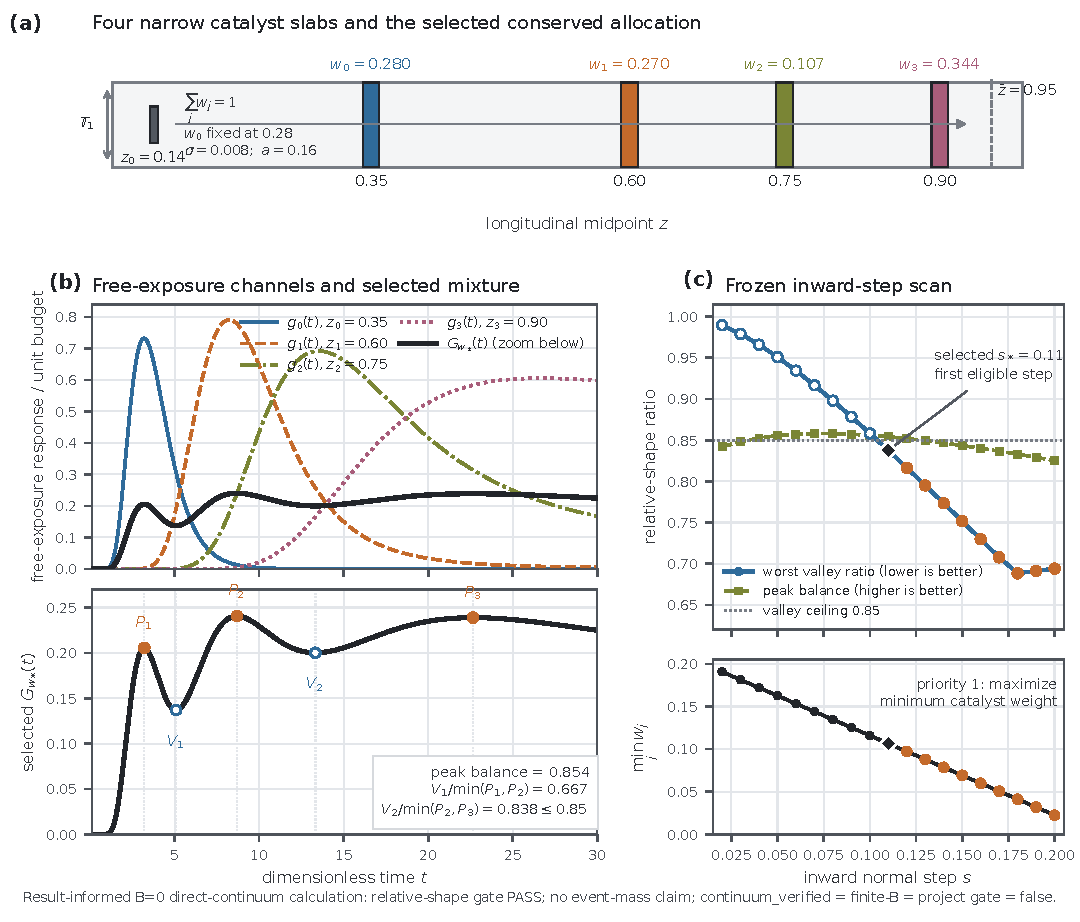
\includegraphics[width=0.94\textwidth]{observable_four_patch.pdf}
\caption{\label{fig:fourpatch}
Exact free-exposure design in the physical-$d=2$ slab quotient.
(a) Four normalized longitudinal catalyst slabs under one conserved installed
budget. (b) The four exact continuum-kernel clocks and their selected $G$
mixture versus dimensionless $t$, with three retained maxima and two
intervening minima. (c) The frozen inward-
step relative-shape scan and its maximum-minimum-weight selection rule.  This
result-informed $B=0$ confirmation is quadrature-converged but is not an
interval-global root certificate, a positive-event-mass statement, or a
finite-$B$ killed-Doi computation.}
\end{figure*}

Coarse, primary, and fine quadratures agree in cusp time within
$\FourPatchCuspTimeSpread$ and in weights within $\FourPatchWeightSpread$; the
primary/fine scaled-quartic difference is $\FourPatchFourthDifference$.  A separate
polar-disk quadrature agrees with the half-chord contact integral within
$\FourPatchPolarDifference$ at four fixed times; primary/fine selected-root
times agree within $\FourPatchRootDifference$.  These checks
support \status{numerically confirmed---exact free-exposure kernel}.  They do not supply
interval-exhaustive root isolation, a positive-$B$ persistence radius, or an
independent killed-PDE solver; the machine-readable flags
\texttt{continuum\_verified}, \texttt{finite\_B\_Doi\_verified}, and
\texttt{project\_gate\_passed} therefore remain false.

\subsection{Physical-d=3 exact sphere-kernel analogue}

We next keep the same longitudinal transport, initial and catalyst bumps,
centres, contact radius, period, and affine slice, but replace the one
periodic relative coordinate by two.  Contact is the true sphere in
$\mathbb R\times\mathbb T_W^2$, and the full-budget slab factor is $1/W^2$.
Both transverse relative coordinates start from independent compact bumps of
half-width $0.004$ centred at zero.  The exact Fourier--Bessel sphere kernel
gives
\begin{align}
 t_c^{(3)}&=\DThreeCuspTime,\nonumber\\
 \bm w_c^{(3)}&=(\DThreeCuspWeightOne,\DThreeCuspWeightTwo,\nonumber\\[-2pt]
 &\qquad \DThreeCuspWeightThree,\DThreeCuspWeightFour),\nonumber\\
 (t_c^{(3)})^4G_{tttt}/G&=\DThreeScaledFourth,\nonumber\\
 \sigma_{\min}/\sigma_{\max}&=\DThreeSvdRatio.
\label{eq:dthreecusp}
\end{align}
All cusp weights are interior and the unfolding has rank two.  Of the 19
frozen inward steps, \DThreeEligibleCount\ pass every relative-shape gate;
the predeclared priority selects $s=\DThreeSelectedStep$ and
\begin{equation}
 \begin{split}
 \bm w_*^{(3)}={}&(\DThreeSelectedWeightOne,\DThreeSelectedWeightTwo,\\[-2pt]
 &\quad \DThreeSelectedWeightThree,\DThreeSelectedWeightFour).
 \end{split}
\label{eq:dthreeselected}
\end{equation}
On the same $[0.1,100]$, spacing-$0.002$ floating-point screen, the retained
alternating roots are
\begin{equation}
 \begin{split}
 &t_1=\DThreeRootOne\ ({\rm max}),\quad
 t_2=\DThreeRootTwo\ ({\rm min}),\\
 &t_3=\DThreeRootThree\ ({\rm max}),\quad
 t_4=\DThreeRootFour\ ({\rm min}),\\
 &t_5=\DThreeRootFive\ ({\rm max}).
 \end{split}
\label{eq:dthreeroots}
\end{equation}
The peak-height ratio is \DThreePeakRatio, and the two valley ratios are
\DThreeValleyOne\ and \DThreeValleyTwo.  Thus the exact sphere-kernel shape
retains three relative-prominence-qualified maxima, although its second-valley
margin below $0.85$ is only about $0.0052$ and is a genuine robustness warning
(Fig.~\ref{fig:d2d3shape}).

Fine-to-primary differences are $\DThreeCuspTimeDifference$ in cusp time,
$\DThreeWeightDifference$ in weight max norm, $\DThreeFourthDifference$ in the
scaled fourth derivative, and $\DThreeRootDifference$ in the largest selected
root time.  A direct spherical-coordinate quadrature of the pointwise product
of one OU and two periodic heat kernels---which does not use the Bessel disk
tensor---agrees at four fixed times within $\DThreeSphericalDifference$.  This
is an independent representation of the free kernel, not an independent PDE
solver.  The calculation is result-informed and $B=0$; its interval,
finite-$B$, independent-solver, and project flags remain false.

\begin{figure*}[t]
\centering
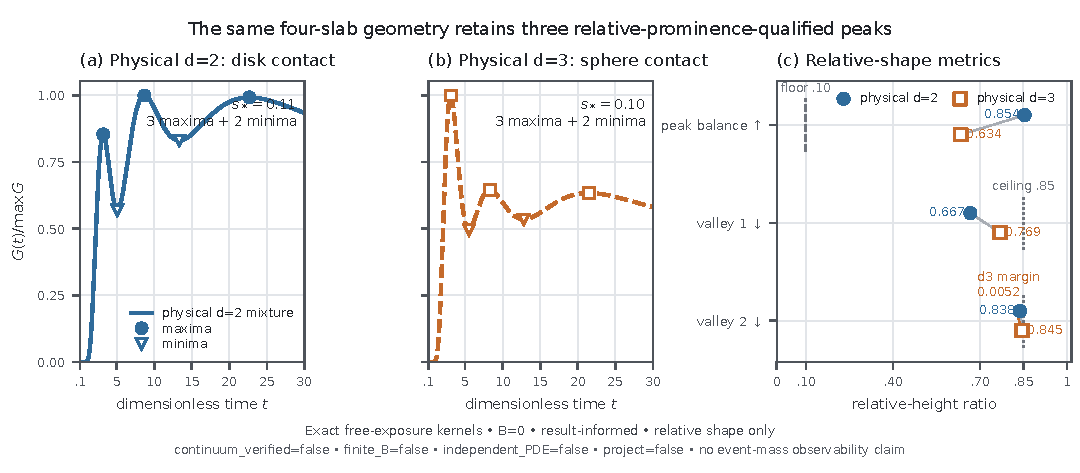
\includegraphics[width=0.96\textwidth]{d2_d3_four_patch.pdf}
\caption{\label{fig:d2d3shape}
Dimension comparison for the same four-slab centres, transport, contact radius,
and frozen selection protocol.  (a) The physical-$d=2$ disk-contact and
(b) physical-$d=3$ sphere-contact selected dimensionless-time $B=0$
free-exposure curves, each normalized only for shape comparison.  Their
selected allocations differ
because each dimension applies the frozen inward-step rule to its own exact
kernel.  (c) Relative peak-balance and valley ratios against the declared
shape thresholds.  Both dimensions retain three qualified maxima, but the
$d=3$ second-valley margin is only $0.0052$.  This result-informed comparison
does not establish positive event mass, finite-$B$ persistence, an independent
killed-PDE solve, or a project gate.}
\end{figure*}

\subsection{$B=0$ finite-volume bridge and discrete history}

A separate result-informed $B=0$ bridge uses the same centres but broader
patch and initial half-widths $0.04$ and $0.02$.  Its exact unbounded-kernel
cusp is at $t=\BroadBZeroCuspTime$, with scaled fourth derivative
$\BroadBZeroScaledFourth$ and unfolding singular-value ratio
$\BroadBZeroSvdRatio$.  A mesh-robustness rule, distinct from the exact-only
selection, chose inward step $s=\BroadBZeroSelectedStep$ and weights
$(\BroadBZeroSelectedWeights)$.  On the one fixed reflecting box of
Eq.~\eqref{eq:g1box}, odd cubic meshes $N=65,97,129,193$ all retain five
alternating sign-changing roots; cusp-time errors decrease as
$\BroadBZeroCuspErrors$, and maximum root-time errors as
$\BroadBZeroRootErrors$.  The two finest meshes also pass the declared
relative peak/valley gates.  This is \status{result-informed $B=0$ numerical
bridge}, not a preregistered discovery, interval certificate, positive-$B$
Doi result, unbounded-box limit, physical-$d=3$ calculation, or project gate.
It does not replace the frozen half-width-$0.008$ chain above.

\subsection{A fixed positive-budget multimodal point}

The exact $B\downarrow0$ calculation was used to choose the broad support
family and the allocation $(\PositiveBWeights)$.  With these physical inputs
held fixed and no positive-budget refit, we evaluated the killed-Doi law at
$B=\PositiveBBudget$ in the same reflected box on the odd meshes
$N=\PositiveBMeshOne$ and $N=\PositiveBMeshTwo$.  Both calculations retain
the max--min--max--min--max topology among five retained roots on the saved
root screen $t\leq35$, and the paired root times differ by at most
\PositiveBMaximumRootDifference.  Peak ratios lie in
$[\PositiveBPeakRatioRange]$; the early and late valley ratios lie in
$[\PositiveBValleyOneRange]$ and $[\PositiveBValleyTwoRange]$.  Partitioning
reaction probability at the two valleys gives the three basin-mass ranges
$[\PositiveBBasinOneRange]$, $[\PositiveBBasinTwoRange]$, and
$[\PositiveBBasinThreeRange]$ through $t=\PositiveBFinalTime$.  Final survival
lies in $[\PositiveBFinalSurvivalRange]$; the largest basin-mass and survival
differences are $\PositiveBMaximumMassDifference$ and
$\PositiveBFinalSurvivalDifference$.

\begin{figure*}[t]
\centering
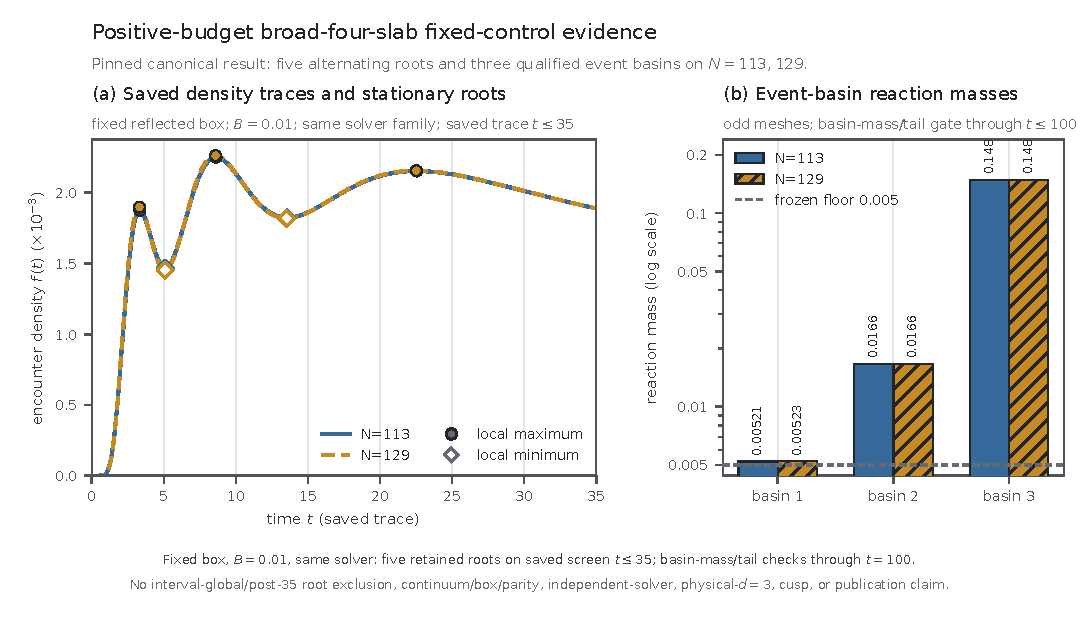
\includegraphics[width=0.98\textwidth]{positive_b_broad_four_slab}
\caption{\label{fig:positiveBfixed}
Fixed-control positive-budget evidence in one broad physical-$d=2$ family.
(a) Saved density traces and the five alternating stationary roots on two odd
finite-volume meshes on the saved root screen $t\leq35$.  (b)
Valley-partitioned reaction masses and tail checks through $t=100$; all six
basin masses exceed the frozen $0.005$ numerical floor.  No interval-global
or post-$35$ root exclusion is claimed.  The
$B\downarrow0$ design fixed the allocation before these positive-$B$
calculations.  The comparison uses one reflected box and one solver family;
it is not a parity, box, continuum, allocation-cusp, independent-solver, or
physical-$d=3$ result.}
\end{figure*}

For one unchanged positive-budget control, this calculation establishes at
least three event-mass-qualified modes in the valley-partitioned sense through
$t=100$, based on five retained roots on the saved screen $t\leq35$; it does
not exclude additional extrema after $t=35$.  The first basin clears the
numerical floor by only $4.23\%$, and the worst valley ratio is
\PositiveBWorstValleyRatio\ against the $0.85$ ceiling.  These tight
margins make parity/alignment, box, and independent-method continuation
scientifically necessary; two odd meshes in one box cannot establish an
unbounded or continuum limit, and one control cannot establish a cusp.

An earlier three-slab, $207\,025$-state free-exposure diagnostic had a
well-conditioned local cusp but no sampled trimodal control: the complete
$0.01$ simplex contained 4696 one-mode and 455 two-mode controls.  Its shallow
extra pair motivated the four-channel construction; it is retained as audit
history rather than promoted as physical trimodality evidence.

The implemented cell-centred solver uses Scharfetter--Gummel longitudinal
fluxes, periodic transverse diffusion, cell-integrated smooth bumps, and
adaptive circle--rectangle contact fractions checked cell by cell against an
independent order-128 Gauss--Legendre construction.  Its current
$25^3=15\,625$-state smoke passes 42 stage-specific gates (38 reusable
foundation gates and four solver gates), including:
\begin{itemize}
\item full-budget relative error $1.85\times10^{-16}$, maximum patch-integral
  error $4.44\times10^{-16}$, and endpoint-budget error
  $3.70\times10^{-16}$;
\item maximum per-cell contact-reference error $2.89\times10^{-15}$ and
  centroid magnitude $5.96\times10^{-17}$;
\item exactly zero discretized initial contact mass;
\item free row-sum and killed mass-balance errors
  $2.69\times10^{-15}$; and
\item dense--sparse semigroup discrepancy $4.41\times10^{-15}$ and relative
  finite-difference jet discrepancies no larger than $1.75\times10^{-8}$.
\end{itemize}
These results are exact algebraic invariants of the assembled discrete
operator and an \status{implementation smoke pass} for the implementation.
They are not a continuum-kernel or continuum-PDE confirmation.  The
subsequent G1b-informed but prospectively frozen
$65\times65\times49=207\,025$-state G1c discovery line propagated eleven
controls on $t\in[0,80]$ with spacing $0.25$, using the generator actions
$K,\Tkill K,\Tkill^2K,\Tkill^3K$.  Every control retained exactly one
sign-changing root of $f_t$ on this screen, a nondegenerate density maximum.
No near-zero extremum or adjacent-
control sign bracket was found.  At one control, $\theta=0.7$, an unmatched
late maximum--minimum pair of $f_t$ triggered the predeclared manual-review
guard.  Both extrema remained below zero; the late maximum was
$-1.3839\times10^{-3}$ and its dimensionless height was $0.51295$, compared
with the discovery cutoff $0.05$.

A separately frozen, explicitly post-result calculation repeated that control
with time spacing $0.05$.  It reproduced the four $f_t$ extrema and exactly
one density maximum; the extra local maximum was
$-1.3837\times10^{-3}$.  Common-time observable discrepancies from the formal
run were at most $5.22\times10^{-14}$.  This is a resolved negative derivative
wiggle, not a fold or a second mode.  Because the original protocol also
required complete adjacent-control extremum matching before declaring the line
empty, the formal line action remains inconclusive rather than being
retroactively relabelled.

\subsection{A result-informed finite-budget finite-grid fold}

A G1b-informed but prospectively frozen full-simplex experiment evaluated
\GOneCControlCount\ triangular-lattice controls and all \GOneCEdgeCount\
neighboring edges at $B=0.6$.  On the frozen $t\in[0,80]$, $\Delta t=0.25$
screen it found \GOneCSeedCount\ strict-interior interpolated seeds;
post-result topology review separated 45 equal-retained-root-count matching
ambiguities from eight edges with one versus three retained sign-changing
roots.
A deterministic largest-minimum-weight rule selected only the segment
\begin{equation}
 \bm w(\lambda)=(0.2,0.1\lambda,0.8-0.1\lambda).
\label{eq:g1dsegment}
\end{equation}
The segment was selected after G1c.  A result-informed, post-G1c augmented
state/sensitivity solve whose numerical choices were frozen before execution,
but which was not a preregistered discovery, solves $f_t=f_{tt}=0$ on the
unchanged bounded-box $207\,025$-state mesh and gives
\begin{align}
 t_f&=\GOneDFoldTime, &
 \lambda_f&=\GOneDFoldControl,\nonumber\\
 \bm w_f&=(\GOneDFoldWeightOne,\GOneDFoldWeightTwo,\nonumber\\
 &\hspace{2.9em}\GOneDFoldWeightThree),\nonumber\\
 f(t_f)&=\GOneDFoldDensity.
\label{eq:g1dfold}
\end{align}
The scaled fold jet is
\begin{align}
 tf_t/f&=\GOneDScaledFt,
 &t^2f_{tt}/f&=\GOneDScaledFtt,\nonumber\\
 t^3f_{ttt}/f&=\GOneDScaledFttt,
 &tf_{t\lambda}/f&=\GOneDScaledFtlambda,\nonumber\\
 t^2f_{tt\lambda}/f&=\GOneDScaledFttlambda.
\label{eq:g1dfoldjet}
\end{align}
and the corresponding dimensionless Jacobian determinant is
$\GOneDJacobianDeterminant$.
On the frozen G1d $t\in[3,18]$, $\Delta t=0.02$ sign-changing-root screen,
$\lambda_f-0.02$ retains alternating maximum--minimum--maximum roots, whereas
$\lambda_f+0.02$ retains one maximum.  This is not a global root census and
does not exclude even-multiplicity or subgrid pairs.  Exact augmented
sensitivities agree with decreasing-step centred control differences within
the frozen tolerance.  This is
\status{numerically verified---discrete diagnostic} for one finite-budget
finite-grid fold.  It is not a continuum extrapolation, a complete phase
map, a cusp, or a trimodality result.

\begin{figure*}[t]
\centering
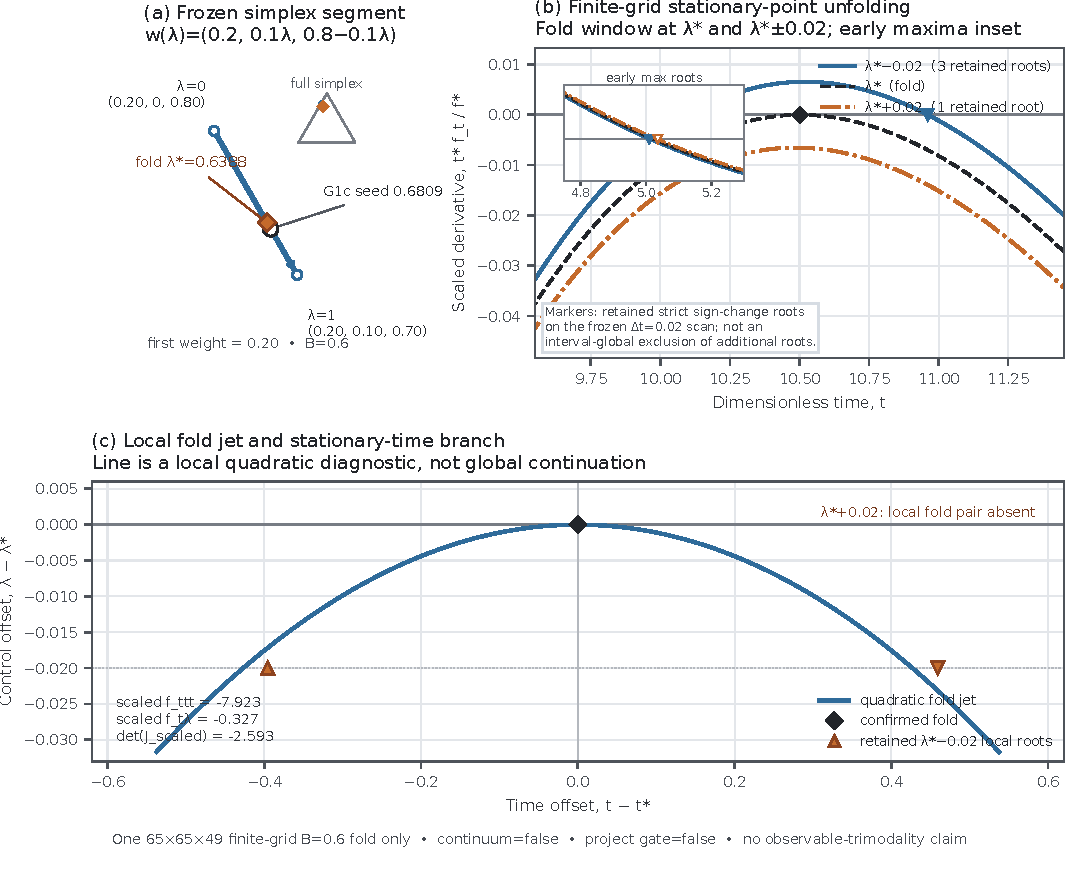
\includegraphics[width=0.90\textwidth]{finite_grid_fold.pdf}
\caption{\label{fig:g1dfold}
One bounded reflected $65\times65\times49$ finite-volume Doi model at
$B=0.6$ only.  The result-informed segment was selected after G1c; its
numerical choices were frozen before the G1d solve, but it was not a
preregistered discovery.  The side panels report retained strict
sign-changing roots on the frozen $t\in[3,18]$, $\Delta t=0.02$ screen.  The
figure is not an interval-global root census, a continuum extrapolation, a
trimodality result, or an independent-solver check.}
\end{figure*}

The next confirmation must converge the entire jet in
Eq.~\eqref{eq:foldjet}, not only the fold coordinates.  Odd/even meshes, box
enlargement, contact quadrature, and an independent off-lattice or
radiation-boundary method must agree.  A finite-$B$ four-slab cusp requires
every entry of Eq.~\eqref{eq:cuspjet}, projected rank two, and five alternating
simple roots with the declared prominence and event-mass floors.

\section{Current gate ledger}\label{sec:status}

\begin{table*}[t]
\caption{\label{tab:gates}
Current evidence.  Each status refers only to the scope in the middle column.}
\small
\begin{tabular}{p{0.15\textwidth}p{0.54\textwidth}p{0.23\textwidth}}
\toprule
Item & Evidence scope & Status\\
\midrule
{\raggedright reduced GIG screens\par} & {\raggedright inherited $m=2,\ldots,6$ roots/cusp; no physical realization\par} & {\raggedright PASS REDUCED ONLY\par}\tabularnewline
{\raggedright multi-rate jet algebra\par} & {\raggedright fixed-support, budget-tangent local theorem\par} & {\raggedright PROVED\par}\tabularnewline
{\raggedright fixed finite $d\ge2$ and finite $m$\par} & {\raggedright admissible monotone/contact-interior targets; $d$-, $m$-, and $\epsilon$-dependent slabs; first $\epsilon$, then $B$; at least $m$; no uniform-in-$d$ claim\par} & {\raggedright PROVED (SCOPED)\par}\tabularnewline
{\raggedright G1a operator smoke\par} & {\raggedright one bounded reflected box; discrete foundations and reference checks\par} & {\raggedright SMOKE ONLY\par}\tabularnewline
{\raggedright narrow four-slab free exposure\par} & {\raggedright result-informed exact unbounded $d=2$ kernels; $B=0$; floating screen and relative shape only\par} & {\raggedright PASS: RESULT-INFORMED $B=0$ SHAPE\par}\tabularnewline
{\raggedright broad four-slab mesh bridge\par} & {\raggedright result-informed $B=0$ exact kernels plus four meshes on one fixed reflected box\par} & {\raggedright PASS: $B=0$ FIXED-BOX BRIDGE\par}\tabularnewline
{\raggedright finite-$B$ fold\par} & {\raggedright post-G1c result-informed mixed jet on one bounded $207\,025$-state grid\par} & {\raggedright PASS: ONE BOUNDED GRID\par}\tabularnewline
{\raggedright fold convergence\par} & {\raggedright odd/even mesh, box enlargement, independent solver\par} & {\raggedright NOT RUN\par}\tabularnewline
{\raggedright positive-$B$ four-slab point\par} & {\raggedright unchanged $B=0.01$ broad allocation; five retained roots on the saved screen $t\leq35$; valley-partitioned basin mass/tail checks through $t=100$; no post-$35$ exclusion; fixed-box odd meshes $N=113,129$\par} & {\raggedright PASS: FIXED CONTROL/TWO MESHES ONLY\par}\tabularnewline
{\raggedright positive-$B$ four-slab cusp\par} & {\raggedright allocation cusp, both folds, and representative modal regions in the same broad family\par} & {\raggedright NOT RUN\par}\tabularnewline
{\raggedright weak-$B$ persistence\par} & {\raggedright bounded and unbounded-weighted compact-time mixed jets; application requires explicit margins\par} & {\raggedright PROVED; APPLICATION NEEDS MARGINS\par}\tabularnewline
{\raggedright global GIG realization\par} & {\raggedright optional physical mixed-jet asymptotic\par} & {\raggedright OPEN\par}\tabularnewline
{\raggedright physical $d=3$ sphere kernel\par} & {\raggedright result-informed exact $B=0$ cusp and relative shape; no killed-PDE event mass\par} & {\raggedright PASS: $B=0$ SHAPE\par}\tabularnewline
{\raggedright positive-$B$ $d=3$ transition\par} & {\raggedright event mass, mesh/box convergence, independent solver\par} & {\raggedright NOT RUN\par}\tabularnewline
\bottomrule
\end{tabular}
\end{table*}

The scoped analytical existence gate is met, and the $B=0$ continuum-kernel
cusp plus the bounded-grid finite-$B$ fold justify continuing the PRR route.
Submission status and stronger headline wording remain withheld until the
same broad family has a finite-$B$ allocation cusp and both folds, the
complete fold/cusp jets and fixed-control event-law features persist under
parity/alignment/box refinement, and an independent method preserves the
positive-budget event-law features.  A two-/three-dimensional headline also
requires separate positive-budget physical-$d=3$ evidence.  The project is
redirected if parity sequences disagree, nondegeneracy vanishes, independent
methods change the topology, or secondary modes fall below the declared
prominence and event-mass floors.

\section{Discussion}\label{sec:discussion}

The organizing object is the zero set of $f_t$ on a conserved-resource control
manifold, not the number of catalyst patches or a particular lattice.  For
every fixed finite integer $d\ge2$ and each prescribed fixed finite $m$, the
direct theorem constructs a $d$- and $m$-dependent longitudinal-slab OU
quotient whose Doi density has at least $m$ nondegenerate maxima after first
choosing a sufficiently small joint
noise/initial-variance/slab-width parameter $\epsilon$ and then a sufficiently
small positive budget.  It does not fix one transport and geometry across
$d$ or $m$, give a uniform-in-$d$ or $d\to\infty$ result, determine the
global number of modes, or provide an event-mass floor; it
deliberately keeps the relative deterministic path inside contact near the
designed peaks.

The result-informed four-slab calculations exhibit three relative-
prominence-qualified maxima and a cusp on the declared floating-point $B=0$
screens for both the physical-$d=2$ disk and physical-$d=3$ sphere kernels.
For the separate broad physical-$d=2$ family, one unchanged allocation at
$B=\PositiveBBudget$ retains three event-mass-qualified modes on two odd
fixed-box meshes in a valley-partitioned check through $t=100$, using five
retained roots on the saved screen $t\leq35$; no post-$35$ or interval-global
root exclusion is available.  Its first-basin and valley margins are tight and
the two meshes use the same solver.  The smaller exact-kernel $d=3$ peak ratio and its
$0.0052$ worst-valley margin identify the three-dimensional design as the more
fragile positive-budget test.  The post-G1c G1d
calculation shows an interior fold at $B=0.6$ on one bounded reflected
finite-volume model.  Neither numerical result closes the other's missing
limit.

The decisive remaining physics is whether fixed-budget allocation coordinates
produce a same-family cusp and both folds, whether the resulting jets and
representative event laws survive parity/alignment/box continuation, and
whether an independent off-lattice killed process preserves the unchanged-
control features within quantified uncertainty.  Positive-budget $d=3$ is a
separate later branch rather than evidence borrowed from the exact $B=0$
sphere kernel.  Further reduced-clock scans do not address these gates.

\begin{acknowledgments}
Funding and computational-resource statements are pending explicit author
confirmation.  Author order, companion-manuscript disclosure, data/code
availability, and archival identifiers remain hard release gates.
\end{acknowledgments}

\appendix

\section{Tail and localization estimates for the direct theorem}
\label{app:directproof}

This appendix records the estimates behind the direct physical theorem.  The
midpoint OU process in Eq.~\eqref{eq:narrowou} has variance
$\epsilon^2s^2(t)$, where
\begin{equation}
 s^2(t)=s_0^2\e^{-2\gamma t}
 +\frac{D_0}{2\gamma}(1-\e^{-2\gamma t}).
\label{eq:midvariance}
\end{equation}
Its invariant variance is $\epsilon^2D_0/(2\gamma)$.  Direct comparison of
Gaussian exponents shows that the declared Gaussian initial density belongs to
$L^2(\pi_\epsilon^{-1})$ precisely when its variance is less than twice the
invariant variance, giving $s_0^2<D_0/\gamma$.  For the longitudinal relative
OU process, the variance coefficient is
\begin{equation}
 u_0^2\e^{-2\gamma t}
 +\frac{2D_0}{\gamma}(1-\e^{-2\gamma t}),
\label{eq:relvariance}
\end{equation}
and the analogous condition is $u_0^2<4D_0/\gamma$.  A wrapped Gaussian is
square integrable against the uniform torus measure for every fixed positive
$\epsilon$.  These observations justify the weighted-space corollary in
Eq.~\eqref{eq:weightedspace}; none is uniform as $\epsilon\downarrow0$.

Let $I_*$ be the union of the target-time neighborhoods and suppose the
deterministic relative mean is at least distance $\eta>0$ inside the contact
ball there.  The relative transition law is a wrapped Gaussian with covariance
$\epsilon^2\Sigma_R(t)$, where $\Sigma_R$ and its time derivatives are bounded
and $\Sigma_R$ is uniformly positive definite on $I_*$.  In the product
geodesic distance on $\mathbb R\times\mathbb T_W^{d-1}$, the reverse triangle
inequality places the complement of the contact ball at distance at least
$\eta$ from the mean.  Differentiating each Gaussian lattice image $r$ times
in $t$ gives that image times a polynomial and a fixed power of
$\epsilon^{-1}$.  Fixed-dimensional lattice shells contain only polynomially
many images while their Gaussian distances grow linearly with shell index.
Integrating the resulting summable majorant outside the contact ball yields
\begin{equation}
 \sup_{t\in I_*}
 |\partial_t^r\{c_{d,\epsilon}(t)-1\}|
 \le C_{r,d}\epsilon^{-N_{r,d}}\exp(-q_d/\epsilon^2).
\label{eq:contacttail}
\end{equation}
The condition $a<W/2$ keeps the embedded contact-ball boundary away from the
torus cut locus; no single chart for its complement is assumed.  Termwise time
differentiation is justified by the same uniform shell majorant on the compact
positive-time interval.  All constants may depend on the fixed finite $d$.

Convolving the normalized Gaussian slab in Eq.~\eqref{eq:narrowslabs} with
the midpoint transition density gives Eq.~\eqref{eq:physicalclock} exactly.
For $t=t_j+\epsilon y$, Taylor expansion on fixed $|y|\le L$ gives
\begin{equation}
 \frac{c_j-\mu(t_j+\epsilon y)}{\epsilon}
 =-\mu'(t_j)y+O(\epsilon)
\label{eq:mutaylor}
\end{equation}
in $C^2$.  Smooth composition with the Gaussian formula and
Eq.~\eqref{eq:contacttail} proves the $C^2$ convergence in
Eq.~\eqref{eq:ownclocklimit}.  If $i\ne j$, strict monotonicity implies
$|c_i-\mu(t)|\ge|c_i-c_j|/2$ on the shrinking $j$th interval for all small
$\epsilon$; time differentiation adds only powers of $\epsilon^{-1}$ and
proves Eq.~\eqref{eq:crossclock}.  Exponential cross-channel decay therefore
dominates the own-channel slope and curvature powers uniformly over every
compact simplex-interior weight set.

Finally, after fixing $\epsilon$, all Gaussian catalysts are bounded.  The
compact-time $C^2$ instance of the unbounded weighted-space corollary following
Eq.~\eqref{eq:weakbridge} preserves the two
endpoint-slope signs and strict negative curvature on every certified local
interval.  This supplies one unique nondegenerate positive-$B$ Doi maximum per
target interval.  Opposite derivative signs on consecutive gap endpoints
force at least one interior local minimum, but neither nondegeneracy of those
minima nor absence of additional extrema is asserted.

\bibliography{references}

\end{document}
